\section{WFS DAN WCS}

\subsection{Web Feature Service(WFS)}
Web Feature Service (WFS) merupakan penyedia antarmuka yang memungkinkan permintaan atau request untuk fitur geografis di seluruh web menggunakan panggilan platform-independen. operasi dasarnya termasuk GetCapabilities, DescribeFeatureType dan GetFeature. Seseorang dapat berpikir tentang fitur geografis sebagai "kode sumber" di belakang peta, sedangkan antarmuka WMS atau online pemetaan portal keramik seperti Google Maps kembali hanya gambar, yang akhir-pengguna tidak dapat mengedit atau spasial menganalisis \cite{franto2015integrasi}.
WFS dapat berupa layanan publikasi data geospasial pada tingkat fitur data spasial melalui media web. Disamping penyajian data spasial melalui gambar/image yang dilakukan oleh WMS, klien dapat memperoleh informasi data geospasial hingga ke lever fitur yaitu baik geometri maupun data atributnya. Spesifikasi OGC untuk WFS menggunakan teknologi XML (Extensible Markup Language) dan protokol HTTP (Hyper Text Transfer Protocol) sebagai media penyampaiannya \cite{ayuningtias2014aplikasi}.
Web Feature Service (WFS) merupakan suatu perubahan dalam pembuatan, pertukaran dan modifikasi data informasi geografis dalam internet. Perbedanya dengan WMS terletak pada kemampuan WFS melakukan publikasi data spasial hingga pada tingkatan unsur. Client WFS dapat memperoleh informasi unsur spasial dalam bentuk vektor, baik pada tingkatan geometri maupun atributnya. Salah satu format data WFS yang paling sering digunakan adalah GeoJSON. GeoJSON menurut situs resminya geojson.org adalah suatu format encoding dari berbagai struktur data spasial. GeoJSON mencakup format-format data geometry berikut: Point, LineString, Polygon, MultiPoint, MultiLineString, dan MultiPolygon \cite{wibowoseminar}.
Meskipun sumber data dalam layanan WFS bervariasi tergantung pada server yang digunakan, database geografis, shapefile adalah suatu keharusan. OGC tidak memberlakukan batasan apa pun pada masalah ini. Selain itu, data yang disajikan adalah GML \cite{putri2018pembuatan}, format pertukaran data berbasis XML. Selain itu, tergantung pada server yang digunakan dalam format berbeda seperti GeoJSON, CSV (Comma Seperated Value), KML, DXF, GeoRSS dapat dilayani.

Dengan WFS, tidak ada aliran data langsung dari server ke klien, sehingga data dapat ditransmisikan dari klien ke server. Pengguna dapat mengubah data pada data yang masuk (menyisipkan, memperbarui, menghapus) untuk mengirimkannya ke server dan memperbarui data. Layanan WFS tersebut disebut Transactional WFS atau WFS-T \cite{khair2016pembuatan}. Anda dapat menemukan beberapa server yang melayani WFS di bawah ini.
Feature server adalah,
\begin{enumerate}
\item GeoServer,
\item Server ArcGIS,
\item Server QGIS,
\item MapServer (TinyOWS)
\end{enumerate}

Desktop QGIS:
\begin{enumerate}
\item ArcGIS Desktop (Ekstensi Interoperabilitas),
\item uDig,
\item OpenLayers,
\item Gaia 3,
\item GRASS GIS
\end{enumerate}

Sebuah web mapping server yang dapat mengembalikan data geografis aktual yang terdiri dari gambar peta tersebut. Hal ini memungkinkan pengguna untuk dapat membuat peta mereka sendiri dan aplikasi dari data, untuk mengkonversi data antara format tertentu, dan dapat melakukan manipulasi data geografis baku dilayani. Protokol yang digunakan untuk mengembalikan suatu data fitur geografis disebut Web Fitur Layanan (WFS) \cite{purab2015penyajian}. Pada gambar \ref{labelgambar1} menunjukkan proses dimana WFS mengubah permintaan menjadi respons.

\begin{figure}[htbp]
\centering
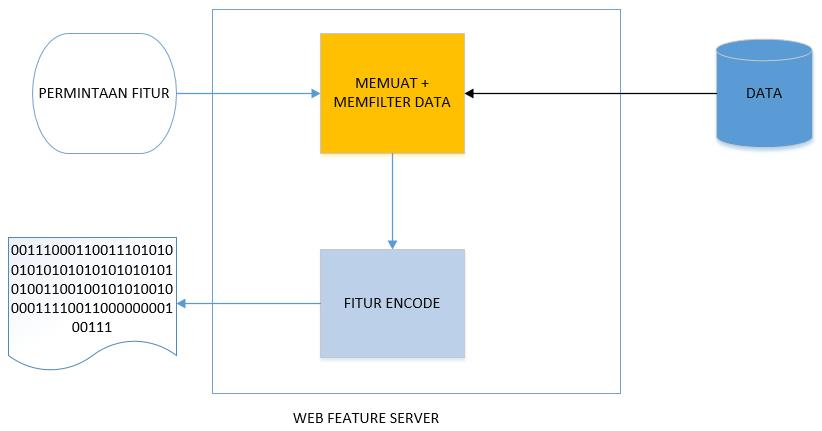
\includegraphics[width=1\textwidth]{pictures/WFS_RSPN}
\caption{menunjukkan bagaimana WFS mengubah permintaan menjadi respons}
\label{labelgambar1}
\end{figure}

Operasi dasar dari WFS antara lain adalah GetCapabilities, DescribeFeatureType dan GetFeature. Operasi yang lebih kompleks tersedia dalam layanan WFS-T (Web Feature Service – Transactional) yang memungkinkan pengguna untuk membuat (menyisipkan), menghapus, memperbarui dan mengunci instance fitur, serta fitur query, Sehingga transaksi dapat disimpan dengan benar dalam datastore (misalnya, SQL RDBMS), semantik transaksi diterapkan.

Tidak seperti OGC Web Map Service (WMS), yang menampilkan gambar peta, layanan WFS menampilkan fitur sebenarnya dengan geometri dan data atribut yang dapat digunakan dalam semua jenis analisis geospasial. Layanan WFS juga mendukung filter yang memungkinkan pengguna untuk melakukan query spasial dan pengaturan data atribut.

Layanan WFS menggunakan Geography Markup Language (GML) untuk menyandikan data fitur. Adapun GML ialah cara untuk merepresentasikan informasi geografis menggunakan XML (Extensible Markup Language) \cite{adityapeluang}.

Web Feature Service merupakan suatu layanan publikasi data geospasial pada tingkat fitur data spasial melalui media web. Disamping penyajian data spasial melalui gambar yang dilakukan oleh WMS, pengguna dapat mendapatkan informasi data geospasial hingga ke lever fitur yaitu baik geometri maupun data atributnya. Spesifikasi OGC untuk WFS menggunakan teknologi Extensible Markup Language dan protocol Hyper Text Transfer Protocol sebagai media penyampaiannya.

\subsection{Cara Membuat Peta Indonesia Melalui WFS}
\begin{enumerate}
\item Pertama yaitu copy kan folder data
\begin{figure}[htbp]
\centering
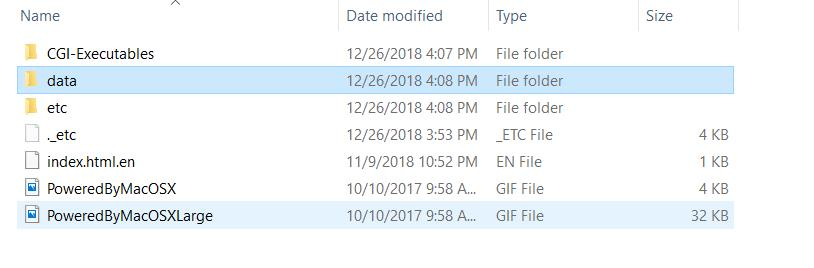
\includegraphics[width=0.5\textwidth]{pictures/Mengcopy_folder_data}
\label{labelgambar 2}
\caption{Mengcopy folder data}
\end{figure}

\end{enumerate}
